% !TeX root = ../main.tex

\chapter{Running the Calibration and Test Script}
\label{chap:Running the Calibration and Test Script}
\section{Overview}

This section will describe how to run and use the Calibration and Test Script, assuming it is configured properly. The following chapters will go into detail on adding new PSC models, and specific details regarding the calibration side and test side of the scripts. 

\begin{center}
	\setlength{\fboxrule}{1.5pt}
	\setlength{\fboxsep}{6pt}
	\fbox{
		\parbox{0.9\textwidth}{
			\textbf{The EEPROM must be configured in the PSC prior to using any of these scripts. Failure to configure the EEPROM, or incorrectly configuring it, will cause issues with the script at even the first menu selection stages.}
		}
	}
\end{center}

\section{Running the Script: Launcher Menu}
To run the script, simply execute the launcher.py script from the repository root directory: \texttt{python3 launcher.py}\\
A menu will appear in your terminal. 
\begin{figure}[H]
	\centering
	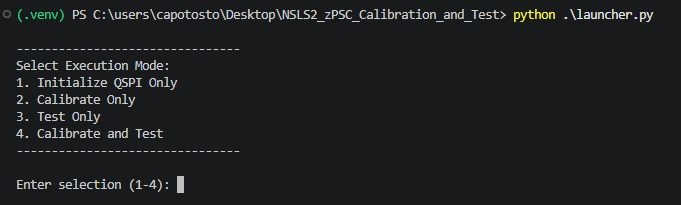
\includegraphics[width=\textwidth]{Python_Screenshots/launcher_menu}
\end{figure}

\newpage \textbf{Choose an option from the menu.}
\begin{enumerate}
	\item Initialize QSPI Only\\
	This option will set the QSPI parameters normally written at the end of calibration, so values such as OVP/OCP, scale factors, and such, will be written to the flash. All gains are written as 1.00, and all offsets written as 0.0. This will overwrite any values stored in QSPI!\\\\This is especially useful for initial testing, where you may want to verify all channels work visually, before committing the time to calibrate and test.
	
	\item Calibrate Only\\
	This option will perform a calibration only, without any tests. This will write all QSPI values at the end of the calibration for each channel.
	
	\item Test Only\\
	This option will perform only the functional tests, without a calibration. This makes no changes to the QSPI. 
	
	\item Calibrate and Test\\
	This option will run a full calibration, and immediately upon completion of the calibration, it will begin the functional test. This allows a calibration and test cycle to be started, and then left alone; so long as the calibration doesn't fail in a way that exits the script, the test can be left unattended for the duration and it will complete without any further user input once it has began (with the exception of the Fast Orbit Feedback Test, which requires a user password)
\end{enumerate}

\newpage
\subsection{Option 1: Initialize QSPI Only}
An example screenshot is provided below.\\
After selecting Menu Option 1, Initialize QSPI Only, the script will sweep the network to detect PSCs. If only one PSC pings, it'll automatically select this unit. If it times out, it'll prompt for the PV prefix of the PSC.\\

The script reads the EEPROM configuration, and trims the option list to those PSCs that match the EEPROM.\\

In this example, a 4Ch High-Stability Fast EIC PSC was being configured, so we chose Option 4. Each channel's QSPI was then written, and the script exited gracefully. 

\begin{figure}[H]
	\centering
	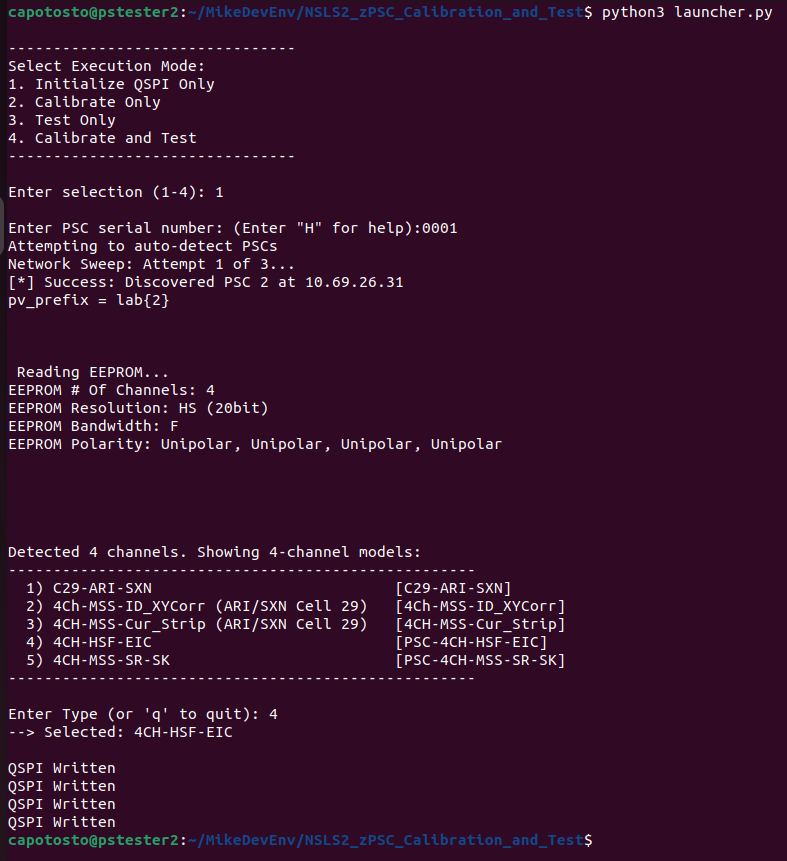
\includegraphics[width=5.75in]{Python_Screenshots/Initialize_QSPI}
\end{figure}
\newpage

\subsection{Option 2: Calibrate Only}
An example screenshot is provided below.\\
After selecting Menu Option 2, Calibrate Only, the script will sweep the network to detect PSCs. If only one PSC pings, it'll automatically select this unit. If it times out, it'll prompt for the PV prefix of the PSC.\\\\
The script reads the EEPROM configuration, and trims the option list to those PSCs that match the EEPROM.\\\\
In this example, a 4Ch High-Stability Slow PSC was being calibrated, so we chose Option 5.\\

A few new prompts will appear:
\begin{enumerate} 
	\item How long do you want to sleep before beginning? (Minutes):\\
	This is asking how long to delay the script's start. For example, if you want the script to wait 15 minutes for the unit to warm up and thermally stabilize, you can simply type 15 and hit \texttt{return}. The script will wait 15 minutes, and then start automatically. 
	
	\item Are the correct tuning boards installed in the ATE? $<$Y/N$>$:\\
	This is a reminder to check and install the correct tuning boards in the ATE. This does not have any effect on the script's function - it does not perform any self tests or verification! It is simply a reminder. Incorrect tuning boards will cause the unit to behave unpredictably.\\
	Install the correct tuning boards before proceeding.
	
	\item Have you run the DMM Self-Calibration within the last 8 hours? $<$Y/N$>$:\\
	This is another reminder prompt. If you haven't, simply perform the auto-cal on the DC Volts range before proceeding. 
	
	\item The calibration script will now take the reigns from here. No further user input is required, the calibration will run, printing results to the terminal as it progresses. Once it completes, it will automatically generate a report text file, timestamped with the model and serial number of the PSC in the filename, located in the \texttt{/cal\_reports} directory. 
\end{enumerate}

\begin{figure}[H]
	\centering
	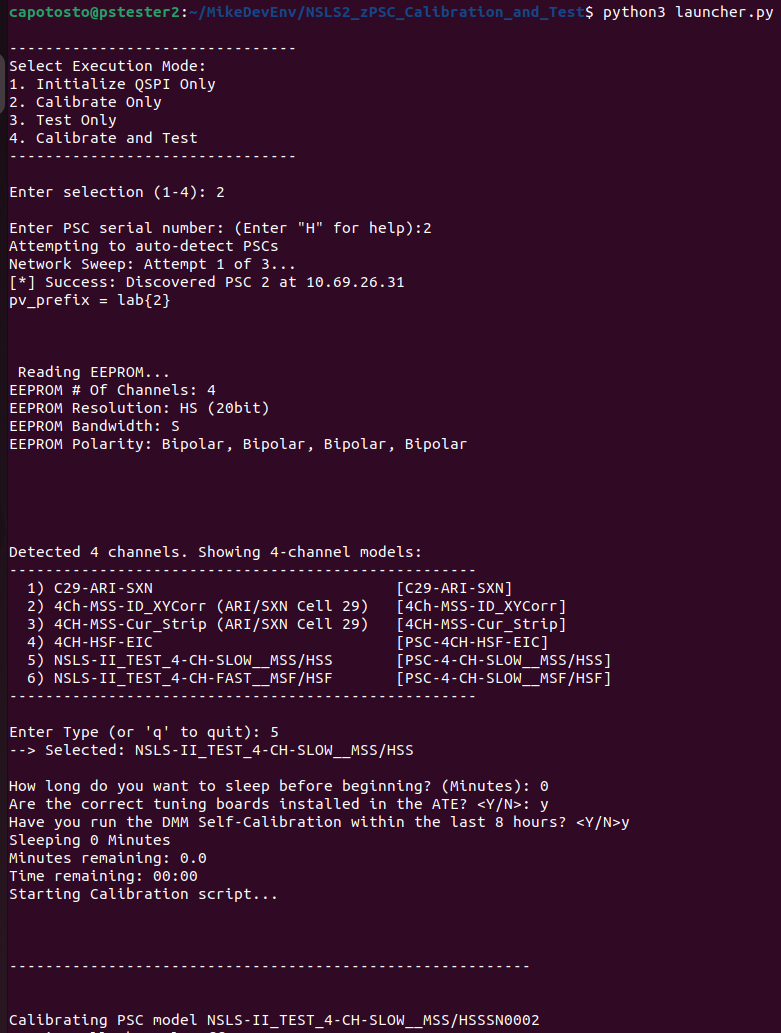
\includegraphics[width=6in]{Python_Screenshots/Calibration_Launch}
	\caption{Menu to launch a Calibrate Only calibration of a PSC}
\end{figure}

\newpage
\subsection{Option 3: Test Only}
An example screenshot is provided below.\\
After selecting Menu Option 3, Test Only, the script will sweep the network to detect PSCs. If only one PSC pings, it'll automatically select this unit. If it times out, it'll prompt for the PV prefix of the PSC.\\\\
The script reads the EEPROM configuration, and trims the option list to those PSCs that match the EEPROM.\\\\
In this example, a 4Ch High-Stability Slow PSC was being tested, so we chose Option 5.\\

A few new prompts will appear:
\begin{enumerate} 
	\item How long do you want to sleep before beginning? (Minutes):\\
	This is asking how long to delay the script's start. For example, if you want the script to wait 15 minutes for the unit to warm up and thermally stabilize, you can simply type 15 and hit \texttt{return}. The script will wait 15 minutes, and then start automatically. 
	
	\item Are the correct tuning boards installed in the ATE? $<$Y/N$>$:\\
	This is a reminder to check and install the correct tuning boards in the ATE. This does not have any effect on the script's function - it does not perform any self tests or verification! It is simply a reminder. Incorrect tuning boards will cause the unit to behave unpredictably.\\
	Install the correct tuning boards before proceeding.
	
	\item The functional test script will now take the reigns from here. No further user input is required, the functional tests will run, printing results to the terminal as it progresses. Once it completes, it will automatically generate a report PDF file, timestamped with the model and serial number of the PSC in the filename, located in the \texttt{/test\_reports} directory.\\\\
	There is one caveat - in that the Fast-bandwidth units will require one input from the user at the very end of the test. The user will be prompted for the SUDO password, as TCPDUMP requires root permission to sniff traffic. The script will pause while waiting for the password, before continuing. This last step requires less than 90 seconds to complete the test and generate the report once the password is entered. 
\end{enumerate}

\begin{figure}[H]
	\centering
	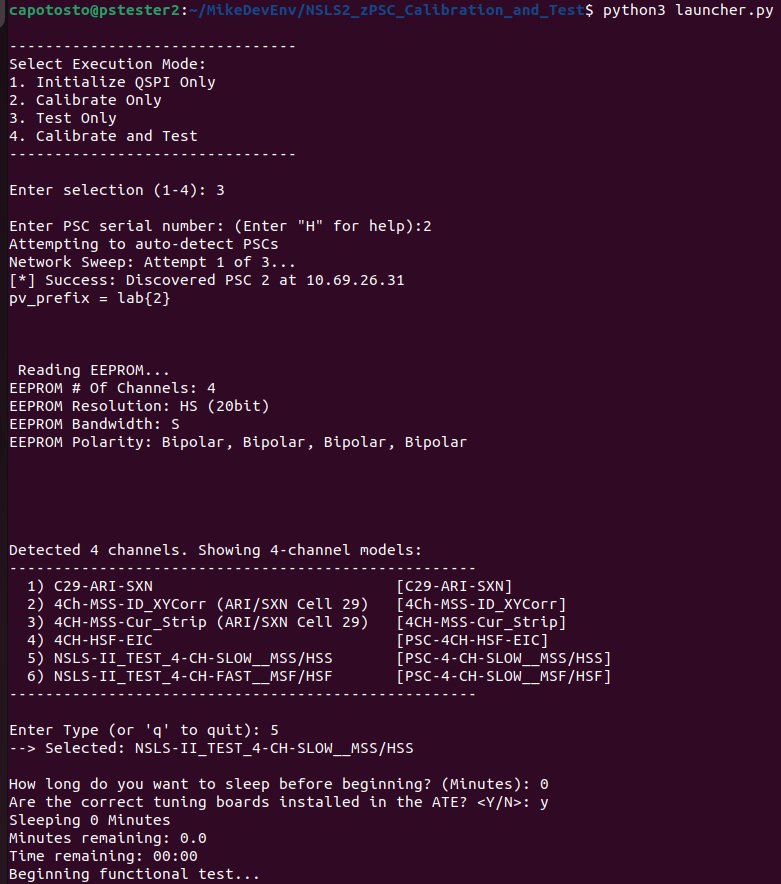
\includegraphics[width=6in]{Python_Screenshots/Test_Launch}
	\caption{Menu to launch a Test Only test of a PSC}
\end{figure}

\subsection{Option 4: Calibrate and Test}
This option will have a menu identical to that of Option 2: Calibrate Only. This simply runs the calibration script, then on completion, runs the test script. No additional figures have been included for this.
